% LaTeX Template for short student reports.
% Citations should be in bibtex format and go in references.bib
\documentclass[a4paper, 11pt]{article}
\usepackage[top=3cm, bottom=3cm, left = 2cm, right = 2cm]{geometry} 
\geometry{a4paper} 
\usepackage[utf8]{inputenc}
\usepackage{textcomp}
\usepackage{subcaption}
\usepackage{graphicx} 
\usepackage{amsmath,amssymb}  
\usepackage{bm}  
\usepackage[pdftex,bookmarks,colorlinks,breaklinks]{hyperref}  
\hypersetup{linkcolor=black,citecolor=black,filecolor=black,urlcolor=black} % black links, for printed output
\usepackage{memhfixc} 
\usepackage{pdfsync}  
\usepackage{fancyhdr}
\pagestyle{fancy}
\usepackage{listings}

\title{GPT-4 sometimes fails to articulate in natural language the rules that it uses for a text-classification task}
\author{Sam Brown}
\date{November 30, 2023}  % Sneaky time-zones :p

\begin{document}
\maketitle


\begin{abstract}
Prompted with a labelled dataset, GPT-4 can sometimes in-context-learn a classification task to $>90\%$ performance.
However, when given the same dataset and asked to articulate a classification rule, GPT-4 sometimes replies with a rule which cannot be the one it is using internally.
At other times, GPT-4 will articulate a rule, yet classify with worse performance than if that rule were implemented.

This report describes experiments with classification on rules based on letter-case, style, language, and length. Sometimes, gentle hints will cause GPT-4 to articulate a good rule, where it seemed unable and confused before.
\end{abstract}

%\tableofcontents

\section{Main findings}

\subsection{Step 1 - In-context learning of classification}


\begin{itemize}

\item GPT-4 can successfully classify data where lines of text are classified as True iff all lower-case.
\item It can discern unexpected patterns in a dataset, based on unanticipated correlations.
\item It can successfully classify short sentences from longer sentences for particular thresholds.
\item It failed at different sentence-length thresholds ($<8$ words rather than $<5$) and at classifying sentences based on whether they contain an odd or even number of words.
\item It can easily distinguish Spanish and English translations of the Bible.
\item It failed to distinguish two English translations with different style.

\end{itemize}


\subsection{Step 2 - Articulation of classification rules}
\begin{itemize}

\item GPT-4 can successfully classify data where lines of text are classified as True iff all lower-case,
yet when asked to articulate a classification rule it describes rules with much worse performance.

\item Given a hint (e.g. ``consider the letter case"), GPT-4 can describe rules with performance matching its unarticulated classification.

\item Hinting is successful enough at prompting articulation of successful rules that multi-choice was not explored.

\item Sometimes the articulated rule will be unexpected, yet still perform well, due to unexpected correlations in the dataset.

\item Some light Chain-of-Thought was prompted, without noticeable improvement.

  \item Articulation of Bible-version rule seems better than classification performance

\end{itemize}




\section{Lower-case}

\subsection{Summary}
\begin{itemize}
  \item Started by scraping lines from Shakespeare play, and classifying based on which were already fully lower-case.
  \item found that there were correlations which were used \& articulated.
  \item decorrelated the dataset, GPT could classify but had difficulty articulating.
  \item by default, articulated rules perform either randomly, or overfit to training examples.
  \item hinting greatly improves articulation. Success of hinting led me not to do multi-choice.
  \item Chain-of-thought did not help much, but I only asked it to ``show your thinking step by step". Better success might have come from giving few-shot examples of successful CoT.
  \item Most important take-away: default unhinted classification is better than the performance of the rules which GPT-4 articulates without hinting.

\end{itemize}

\subsection{Detail}

A dataset was created from the text of \emph{The Comedy of Errors} by Shakespeare.
Lines of the plays are sometimes already fully lower-case, and so a balanced dataset can be made using an equal number of fully-lower-case lines (labelled 'True') and lines with a capital letter (labelled 'False'), see Figure \ref{fig:unaltered-lines}.


        
\begin{figure}
\centering
\begin{subfigure}{0.49\textwidth}
    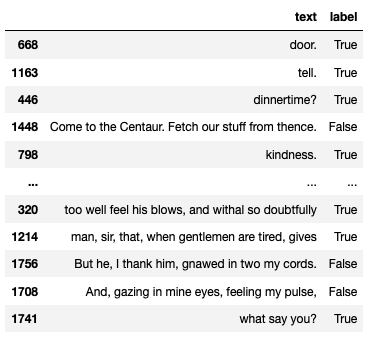
\includegraphics[width=\textwidth]{images/balanced-organic-comedy-of-errors-lines.png}
    \caption{Unaltered data, with many fragments}
    \label{fig:unaltered-lines}
\end{subfigure}
\hfill
\begin{subfigure}{0.49\textwidth}
    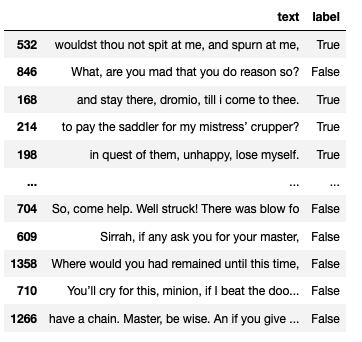
\includegraphics[width=\textwidth]{images/balanced-forced-comedy-of-errors-lines.png}
    \captionsetup{justification=centering}
    \caption{Half the lines forced to lower-case\\(n.b. lower-case `i' in $\#168$)}
    \label{fig:altered-lines}
\end{subfigure}
\caption{
In \eqref{fig:unaltered-lines}, the lines are classified based on whether they are \emph{already} lower-case; this correlates strongly with line length and fragmentation.
In \eqref{fig:altered-lines}, previously mixed-case are forced to lower-case (previously all-lower-case are dropped) and this correlation is removed.
}
\end{figure}


When this dataset is given in a prompt to GPT-4 it quickly learns to classify with ${\sim}90\%$ accuracy, see Figure \ref{fig:corr_class}, after seeing about 25 examples .\footnote{
GPT-3.5-turbo was also explored for this first task, but left out of later experiments due to its worse performance.}
To prompt, \texttt{\{"role": "user"\}} and \texttt{\{"role": "assistant"\}} messages are used for the inputs and labels respectively; no system prompt is used during the default classification task.

GPT-4 was then asked to generate an explanation using a system prompt (see Listing \ref{lst:articulate}).

\begin{lstlisting}[caption={A basic system prompt can lead GPT-4 to articulate classification rules}, captionpos=b, frame=single, label={lst:articulate}]
You are given some statements, which are labelled with categories.
Describe the classification rule.
\end{lstlisting}


However, GPT-4 unexpectedly described a unintended aspect of the dataset: that lines with only lower-case letter (and therefore classified as `True') were more likely to be fragments or partial sentences (see Figure \ref{fig:fragment-reason}). This was confirmed manually, see Figure \ref{fig:wc-corr}, and results from line-breaks in the Shakespeare play's prose.


\begin{figure}
  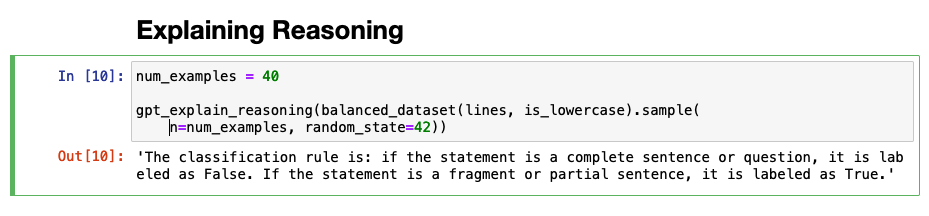
\includegraphics[width=\linewidth]{images/fragment-reason.png}
  \caption{GPT-4 identifies unexpected features in the data.}
  \label{fig:fragment-reason}
\end{figure}




To correct for this, any already-lower-case lines were dropped, and half of the remaining data was random cast to all-lower-case (see Figure \ref{fig:altered-lines}).



\begin{figure}
\centering
\begin{subfigure}{0.49\textwidth}
    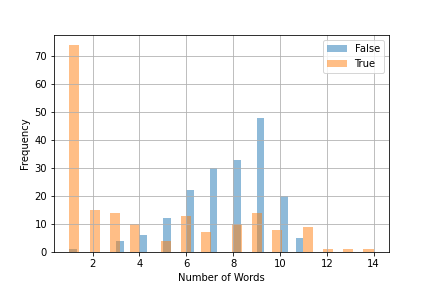
\includegraphics[width=\textwidth]{images/word-count-correlating-with-lowercase-class.png}
    \caption{Correlation in the organic dataset}
    \label{fig:wc-corr}
\end{subfigure}
\hfill
\begin{subfigure}{0.49\textwidth}
    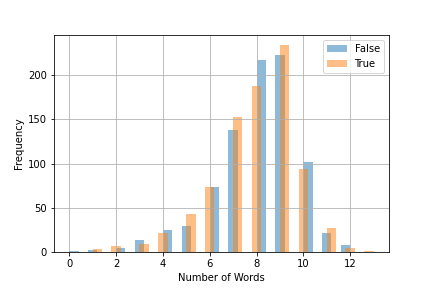
\includegraphics[width=\textwidth]{images/word-count-decorrelated-from-lowercase-class.png}
    \caption{Decorrelated data}
    \label{fig:wc-decorr}
\end{subfigure}
\caption{
Word-counts of lines of Shakespeare, classified by being entirely lower-case (True) or not (False).
In \eqref{fig:wc-corr}, lines of Shakespeare are classified based on whether they are \emph{already} lower-case; this correlates strongly with line length and fragmentation.
In \eqref{fig:wc-decorr}, the dataset is modified to remove this correlation.
}
\end{figure}


GPT-4 was also able to classify this decorrelated data, though it took ${\sim}50$ examples, about twice as many as before (see Figure \ref{fig:corr_class}).


\begin{figure}
\centering
\begin{subfigure}{0.49\textwidth}
    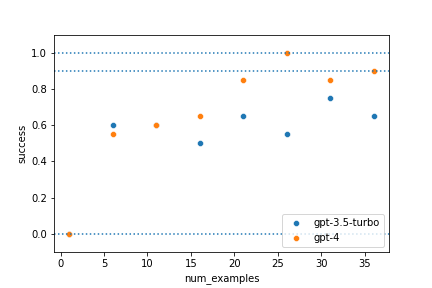
\includegraphics[width=\textwidth]{images/lowercase-classification-with-correlation.png}
    \caption{With correlated data}
    \label{fig:corr_class}
\end{subfigure}
\hfill
\begin{subfigure}{0.49\textwidth}
    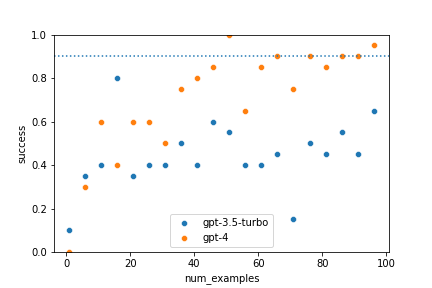
\includegraphics[width=\textwidth]{images/lowercase-classification-without-correlation.png}
    \caption{With decorrelated data}
    \label{fig:decorr_class}
\end{subfigure}
\caption{
GPT performance on classifying lines of Shakespeare based on whether the line is upper- or lower-case.
In (a), the lines are classified based on whether they are \emph{already} lower-case; this correlates strongly with line length and fragmentation, and so these latter features are what is learned by the GPT classifier, and so GPT-4 can successfully classify by ${\sim} 25$ examples.
In (b), this correlation is removed, and GPT-4 requires ${\sim} 50$ examples to successfully classify lines.
}
\end{figure}


However, this time the classification rules articulated by GPT-4 seemed confused (see Figure \ref{fig:forced-reason}).


\begin{figure}
  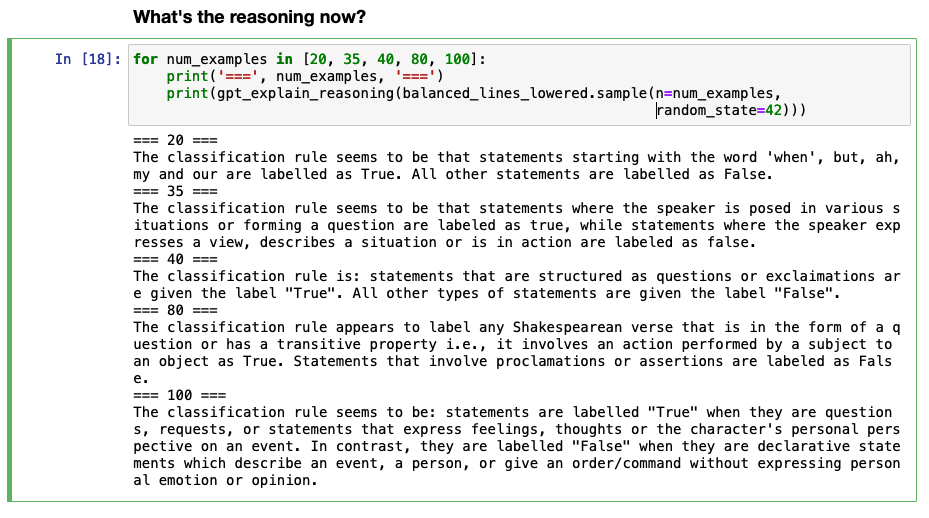
\includegraphics[width=\linewidth]{images/forced-comedy-of-errors-reason.png}
  \caption{GPT-4 continues not to mention letter-casing, and seems confused.}
  \label{fig:forced-reason}
\end{figure}


Since GPT-4 had identified real unexpected features before, I checked how these confused rules performed, just in case some feature was being found, using a system prompt described in Listing \ref{lst:custom-rule}. It was clear that performance for these rules was generally random (accuracy ${\sim}50\%$) or at times over-fit to the training data (train: ${\sim}70\%$ ; test: ${\sim}50\%$).

\begin{lstlisting}[caption={A system prompt to instruct GPT-4 to use a given classification rule}, captionpos=b, frame=single, label={lst:custom-rule}]
You are a helpful assistant.
You classify statements, outputting only the classification label,
using the following rule: <RULE>
\end{lstlisting}

\subsubsection{Hinting}
Providing a hint in the system prompt (see Listing \ref{lst:hint}) triggered GPT-4 to immediately be able to articulate good letter-casing-based classification rules (see Figure \ref{fig:hinting-reasons}). Note that while one rule was expected (all lower-case) and found (though not mentioned in the figure), GPT-4 also found that it could predict based on only the first letter: this rule has $98\%$ success in classifying (c.f. $100\%$ for the correct ``all-lowercase" rule).

\begin{lstlisting}[caption={A system prompt containing a hint}, captionpos=b, frame=single, label={lst:hint}]
You are given some statements, which are labelled with categories.
Describe the classification rule.
(Hint: consider the letter case)
\end{lstlisting}


\begin{figure}
  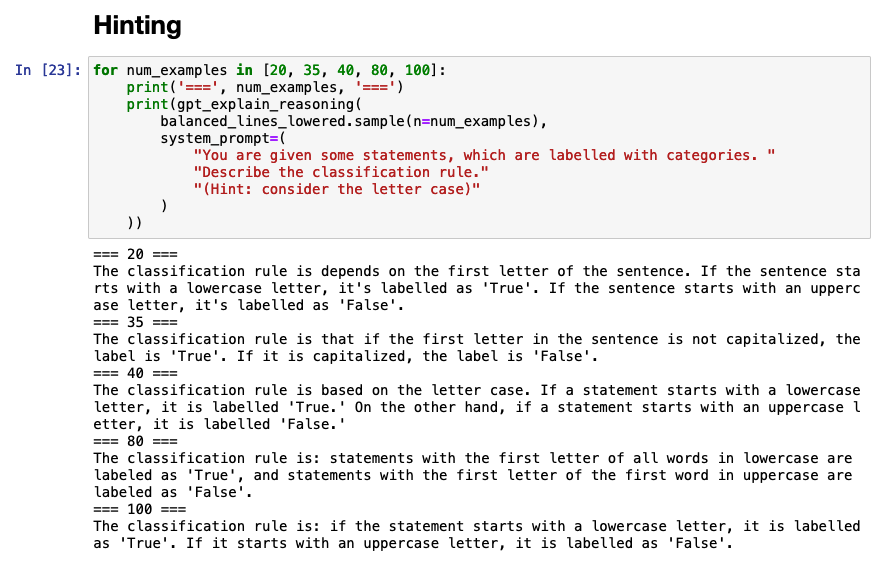
\includegraphics[width=\linewidth]{images/hinting-reasons.png}
  \caption{When the system prompt contains a hint, GPT-4 can reliably identify letter-casing rules. First-letter capitalisation has an accuracy of $98\%$. All-letter capitalisation (found but not shown) has an accuracy of $100\%$.}
  \label{fig:hinting-reasons}
\end{figure}


\subsubsection{Chain-of-Thought}

I tried some very quick Chain-of-Though, using a short system prompt (see Listing \ref{lst:cot}). This didn't help very much, instead leading to waffly but incorrect rules (see the Jupyter notebook for examples).

\begin{lstlisting}[caption={A system prompt attempting to trigger Chain-of-Thought}, captionpos=b, frame=single, label={lst:cot}]
You are given some statements, which are labelled with categories.
Consider at least two possible classification rules,
showing your thinking step-by-step, and choose the most likely.
\end{lstlisting}


\section{Number of words}
Next I wanted to see whether number-of-words was something that GPT-4 could classify on.
Based on the distribution of words in lines of \emph{The Comedy of Errors} (see Figure \ref{fig:wc-hist}), I chose 8 (the median) and 5 as thresholds, and tested three rules:

\begin{itemize}
	\item \texttt{$<5$ words}: ``True iff the statement has fewer than 5 words (space-separated)"
   \item  \texttt{$<8$ words}: ``True iff the statement has fewer than 8 words (space-separated)"
   \item  \texttt{odd}: ``True iff the statement has an odd number of words (space-separated)"
\end{itemize}

Classification performance was good for the first of these ($<5$), but not the second (see Figure \ref{fig:wc-class}).

\begin{figure}
\centering
\begin{subfigure}{0.49\textwidth}
    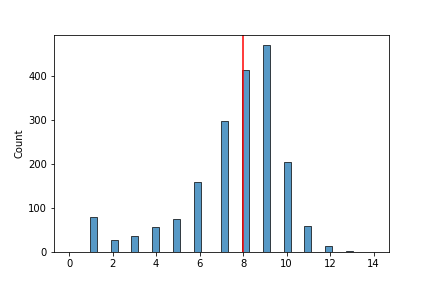
\includegraphics[width=\textwidth]{images/comedy-of-errors-lines-wordcount-histogram.png}
    \captionsetup{justification=centering}
    \caption{
    	Word-counts of lines of Shakespeare in dataset.\\
    	Red line shows the median.
    	}
    \label{fig:wc-hist}
\end{subfigure}
\hfill
\begin{subfigure}{0.49\textwidth}
    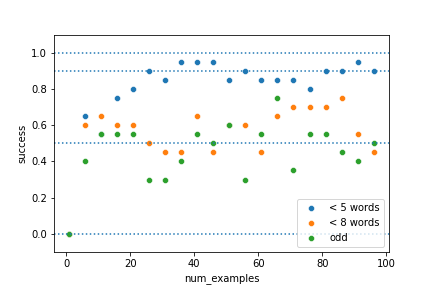
\includegraphics[width=\textwidth]{images/wordcount-classification.png}
    \caption{GPT-4's classification performance}
    \label{fig:wc-class}
\end{subfigure}
\caption{
Figure \eqref{fig:wc-hist} shows the distribution of word-counts in the lines of Shakespeare used as a dataset.
Figure \eqref{fig:wc-class} shows GPT-4's performance in classifying based on three tests, \emph{without hints}. GPT-4 learns to classify lines which are shorter than 5 words long, but has trouble when the threshold is ``8 words long", and when the criteria is ``is the number of words odd or even?".
}
\end{figure}



Exploring the provided reasoning here explained the discrepancy between the performance at two thresholds:
for the shorter threshold the LLM was often detecting the incompleteness of the sentence, focussing on sense rather than composition (see Figure \ref{fig:wordcount-reasons}).



\begin{figure}
  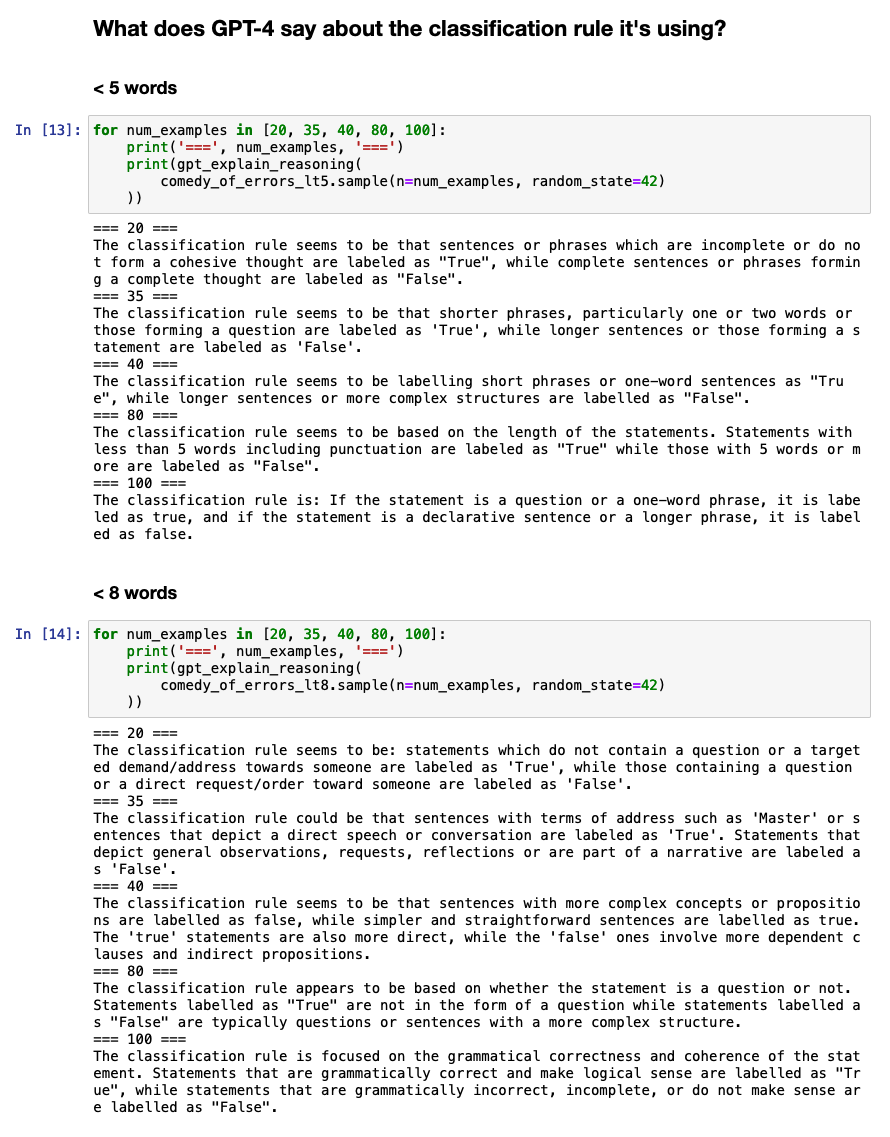
\includegraphics[width=\linewidth]{images/wordcount-reasons.png}
  \caption{Classification rules articulated by GPT-4 for a dataset labelled using word-counting.
  Note that for $<5$ words at $80$ examples, the LLM stumbles on the correct rule.}
  \label{fig:wordcount-reasons}
\end{figure}

Again, hinting (with ``consider the number of words") is enough to trigger GPT-4 into giving more correct rules, although the precise value of the threshold given varies slightly (e.g. $3-4$ for $<5$, $6-7$ for $<8$), possibly due to limited number of examples.

For odd vs even, classification and articulation are both unsuccessful without hinting. See the Jupyter notebook for more details.


\section{Bible version classification (inc. Spanish)}

We now look at three different translations of the Bible:

\begin{itemize}
	\item King James Version (KJV): One of the most famous and historically significant English translations of the Bible, originally published in 1611.
	\item Easy-to-Read Version (ERV): Designed to be easy to read and understand, it's often used for English language learners, children, and people with lower reading skills.
	\item Reina-Valera 1989 (RV): A modern revision of the classic Spanish Protestant translation that aims to preserve the traditional linguistic beauty while updating the language for contemporary readers.
\end{itemize}

Since they are all translations of the same text, the classification datasets are balanced.

Classification results are shown in Figure \ref{fig:bible-class}, and articulated rules for KJV vs ERV are shown in Figure \ref{fig:bible-reasons}.

\begin{itemize}
	\item KJV vs RV: Classification is very quickly reacked at $100\%$ accuracy, and articulated rules quickly identify ``Spanish vs English".
	\item KJV vs ERV: Classification is poor, yet GPT-4 manages to correctly articulate the rule ``direct quote from the Bible [KJV] vs paraphrase".
\end{itemize}

\begin{figure}
  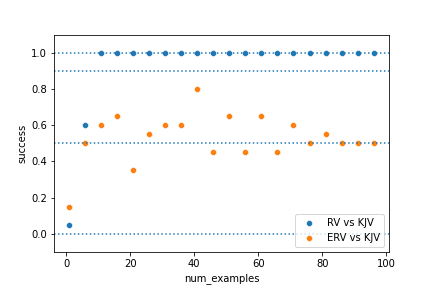
\includegraphics[width=\linewidth]{images/bible-classification.png}
  \caption{GPT-4 very quickly learns to distinguish verses from a Spanish translation of the Bible (Reina-Valera 1989) from those of an English translation (King James Version), but has trouble distinguishing between the King James Version and another English-language translation in a different style (Easy Reading Version).}
  \label{fig:bible-class}
\end{figure}


\begin{figure}
  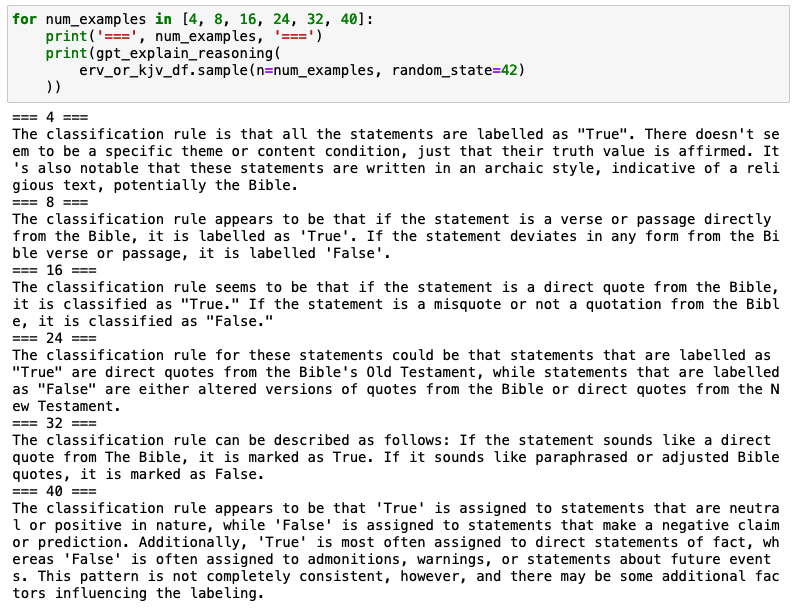
\includegraphics[width=\linewidth]{images/bible-reasons.png}
  \caption{GPT-4 quickly identifies that one class corresponds to ``direct quotes" from the bible (presumably King James Version), but describes ``paraphrasing" rather than identifying the Easy Reading Version.}
  \label{fig:bible-reasons}
\end{figure}

It's surprising to me that it can articulate this rule, but can't seem to use it to get good classification.
This seems to go in the other direction to the lower-case function, where classification without articulation performed better.

If I were to spend more time on this, I'd investigate GPT-4's ability to identify direct quotes from the KJV when directly prompted,
to determine to what extent the poor classification performance comes simply from not having memorised the full KJV.




\bibliographystyle{abbrv}
% \bibliography{references}  % need to put bibtex references in references.bib 
\end{document}
